\section{Méthode de developpement}


\subsection{Cycle Itératif}
La méthode de développement pour le projet tuteuré est plus ou moins imposée. En effet pour pouvoir suivre l'avancement du projet, les tuteurs demandent aux étudiants d'utiliser un cycle itératif (figure \ref{cycle_iteratif}).

\begin{figure}[H]
\centering
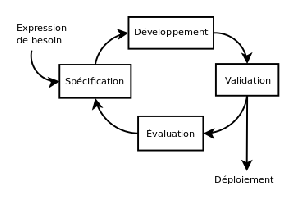
\includegraphics[width=8cm]{images/activite/cycle_iteratif.eps}
\caption{Schéma cycle Itératif}
\label{cycle_iteratif}
\end{figure}

\subsection{Outils de developpement}
Le choix du langage à utiliser était libre, nous avons donc opté pour un langage simple d'utilisation et ayant déjà fait ses preuves : \textbf{Java} (figure \ref{java_logo}).
\\
\\
\\

\begin{figure}[!h]
\centering

\includegraphics[width=8cm]{images/activite/javaLogo.eps}
\caption{Logo Java}
\label{java_logo}
\end{figure}


Nous avons choisi de travailler avec le logiciel \textbf{Éclipse} (figure \ref{eclipse_logo}), un \gls{IDE} pour développer en \textbf{Java}.

\begin{figure}[H]
\centering

\includegraphics[width=8cm]{images/activite/eclipseLogo.eps}
\caption{Logo Éclipse}
\label{eclipse_logo}
\end{figure}

\textbf{Éclipse} est disponible à l'IUT et libre.
La bibliothèque nous permettant de faire des \gls{ihm} est java.swing, un package Java documenté et expliqué par Oracle
\footnote{Tutoriel java.swing : \url{https://docs.oracle.com/javase/tutorial/uiswing/}}

\section{Planification}
Le projet a été découpé en sept itérations de durées variantes (d'une semaine à un mois) en fonction des périodes d'examens et de vacances. 
Chaque itération refactore le code et en ajoute.

\subsection{Itération 1 - 14/11/2016}

\subsubsection{Fonctionnalités et travail réalisé}
\begin{itemize}
\item Connexion à une base de données Oracle.
\item Mode requêtes SQL.
\end{itemize}

\subsubsection{Résultat}
L'utilisateur peut se connecter à une base de données mais il y a des problèmes au niveau des champs de saisies. 
Le mode requête SQL ne fonctionne pas parfaitement.
Cette itération n'a pas de grosse valeur ajoutée pour le client. 
Elle a surtout permis de poser les bases du travail en groupe en posant les bases des outils de collaboration.


\subsection{Itération 2 - 02/12/2016}
\subsubsection{Fonctionnalités et travail réalisé}
\begin{itemize}
\item Correction des bugs sur la fenêtre de connexion et sur le mode Requêtes SQL.
\item Création de tables.
\end{itemize}

\subsubsection{Résultat}
Les bugs signalés sont corrigés et la vue de création des tables fonctionne avec quelques bugs mineurs.
Cette itération est satisfaisante pour le groupe car les attentes ont été respectées.

\subsection{Itération 3 - 15/12/2016}
\subsubsection{Fonctionnalités et travail réalisé}
\begin{itemize}
\item Connexion à MySQL.
\item Correction des bugs sur la fenêtre de création des tables.
\item Suppression des tables.
\item Modification des tables.
\end{itemize}

\subsubsection{Résultat}
Les bugs signalés sont corrigés et la vue de suppression des tables fonctionne.
La modification des tables fonctionne partiellement.
Cette itération est mitigée car la valeur apportée au client n'était pas conséquente. 


\subsection{Itération 4 - 12/01/2017}
\subsubsection{Fonctionnalités et travail réalisé}
\begin{itemize}
\item Correction de bugs sur la fenêtre de modification des tables.
\item CRUD des tuples d'une table.
\end{itemize}

\subsubsection{Résultat}
La fenêtre CRUD fonctionne partiellement (fonctionnalité \textit{update} non-implantée) et quelques bugs sur l'insertion. 
La modification des tables fonctionne partiellement.
Cette itération est peu satisfaisante mais a permis une remise en question de notre organisation. 

\subsection{Itération 5 - 02/02/2017}
\subsubsection{Fonctionnalités et travail réalisé}
\begin{itemize}
\item Correction des bugs sur le CRUD et ajout de la fonctionnalité update.
\item Début de la refonte des classes métiers de l'application.
\end{itemize}

\subsubsection{Résultat}
La fenêtre CRUD fonctionne avec quelques bugs mineurs.
La refonte des classes métiers avait pour but de stocker les différentes informations des tables des bases de données et ainsi limiter les accès à celles-ci.
De plus, les classes métiers devaient permettre de gérer plus facilement le processus de modification des tables. 
La modification de table ne marche plus, mais la refonte des classes métiers va permettre de la faire fonctionner.
Cette itération est satisfaisante puisque la refonte des classes métiers simplifie beaucoup de choses. 

\subsection{Itération 6 - 09/02/2017}
\subsubsection{Fonctionnalités et travail réalisé}
\begin{itemize}
\item Correction des bugs sur la fenêtre CRUD.
\item Fin de la refonte des classes métiers de l'application.
\item Modification des vues de Creation-Supression-Modification des tables pour qu'elles collent aux classes métiers.
\item Création et supression des contraintes (uniques et clées étrangères).
\end{itemize}

\subsubsection{Résultat}
La fenêtre CRUD fonctionne avec quelques bugs mineurs.
La création et la suppression des tables fonctionnent avec les nouvelles classes métiers.
La création et la suppression des contraintes fonctionnent partiellement.
Cette itération est dans la continuité de l'itération 6. 

\subsection{Itération 7 - 20/02/2017}
\subsubsection{Fonctionnalités et travail réalisé}
\begin{itemize}
\item Correction des bugs sur la création et la suppression de contraintes ainsi que sur la fenêtre CRUD.
\item Faire des requêtes graphiques (QBE).
\item Modification de tables.
\item Refactoring.
\end{itemize}

\subsubsection{Résultat}

La modification des tables et le QBE fonctionnent.
La création et la suppression des contraintes fonctionnent avec quelques bugs mineurs.
Cette itération concerne surtout la correction des bugs et la rédaction du rapport. 


\section{Outils de collaboration}

\subsection{Gestionnaire de version}
Les premiers échanges que nous avons eus après l'attribution du sujet se sont concentrés sur le choix du gestionnaire de version que nous allions utiliser au cours du projet. Ce gestionnaire de version permet en autre de :
\begin{itemize}
\item Partager le code source de l'application.
\item Gérer des conflits lors de la modification simultanée d'un fichier.
\item Maintenir l'ensemble des versions d'un ou plusieurs fichiers.\\
\end{itemize}

Etant majoritairement habitué à utiliser Git, c'est vers un dép\^ot \textbf{Github} (figure \ref{github_logo}) que nous nous sommes tourné
\footnote{Site web GitHub : \url{https://github.com/}}.

\begin{figure}[H]
\centering

\includegraphics[width=8cm]{images/activite/githubLogo.eps}
\caption{Logo GitHub}
\label{github_logo}
\end{figure}



\subsection{Répartition des tâches}
Au cours de leurs formations antérieures, certains membres du projet ont utilisé l'outil de gestion de projet \textbf{Trello} (figure \ref{trello_logo}). 
C'est pourquoi nous avons utilisé cet outil pour répartir les tâches.\\

\begin{figure}[H]
\centering

\includegraphics[width=8cm]{images/activite/trelloLogo.eps}
\caption{Logo Trello}
\label{trello_logo}
\end{figure}

\textbf{Trello} permet de découper en \textit{tickets} les différentes t\^aches à réaliser. Ces tickets peuvent \^etres déplacés par les membres du projet dans différentes catégories :

\begin{itemize}
\item \textbf{TODO} - les t\^aches qu'il restent à faire. 
\item \textbf{DOING} - les \^aches en cours de développement.
\item \textbf{TESTS} - les t\^aches en cours de test.
\item \textbf{DONE} - les t\^aches qui sont terminées.\\
\end{itemize}

Chaque membre choisit un ticket dans la partie TODO et le déplace dans DOING. 
Puis lorsqu'il a terminé de développer la fonctionnalité, le ticket va dans TEST et pour finir dans DONE.

\subsection{Communication}
Les outils de communication ont évolué au cours du projet. Nous avons tout d'abord utilisé naturellement la messagerie instantanée que propose \textbf{Facebook}. 
Cette messagerie simple, permet de partager des images ainsi que des documents.
Cependant nous souhaitions pouvoir discuter à l'oral ce que ne permet pas facilement la messagerie de Facebook. 
C'est pour cette raison que nous avons migré sur le logiciel \textbf{Discord} (figure \ref{discord_logo}) qui permet, en plus de la messagerie et de l'échange de documents, de discuter à l'oral ce qui a grandement facilité notre communication.

\begin{figure}[!p]
\centering

\includegraphics[width=10cm]{./images/activite/discordLogo.eps}
\caption{Logo Discord}
\label{discord_logo}
\end{figure}

De plus, nous avons installé un BOT sur le Discord, lié a GitHub, qui écrit un message lors d'une modification du dép\^ot git (figure \ref{bot_discord}).

\begin{figure}[!p]
\centering
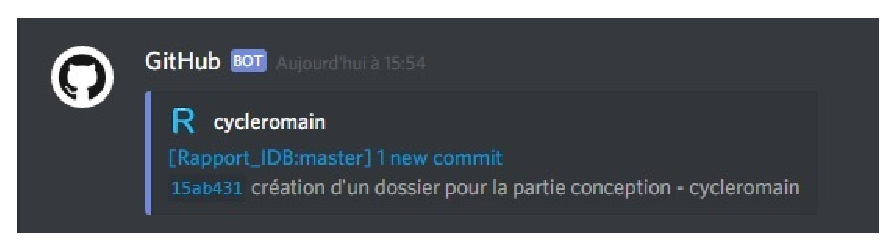
\includegraphics[width=10cm]{./images/activite/bot_discord.eps}
\caption{Message du BOT Discord lié à GitHub}
\label{bot_discord}
\end{figure}



\subsection{Partage de documents}
Tout au long du projet, nous avons produit différents documents qu'il nous a fallu stocker dans un endroit facile d'accès pour tous. 
Nous avons donc créé un dossier sur un \textbf{Google Drive} (figure \ref{googledrive_logo}) et l'avons partagé aux membres du groupe. Ce Drive nous a permis d'échanger et stocker des diagrammes, des pdfs, des documents texte, des maquettes pour les \glspl{ihm}* ainsi que d'autres fichiers que nous voulions conserver.

\begin{figure}[!p]
\centering

\includegraphics[width=10cm]{./images/activite/googleDriveLogo.eps}
\caption{Logo Google Drive}
\label{googledrive_logo}
\end{figure}



